\documentclass{standalone}
\usepackage{tikz}
\usetikzlibrary{angles,quotes}
\begin{document}
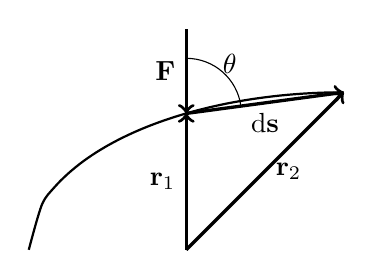
\begin{tikzpicture}[scale=2]
    \draw[-,thick]plot[smooth, domain=-2:0](\x,{(1-(\x)^2/4)^0.5});
    \draw[->,very thick](-1,0)--(-1,0.866)node[midway, left]{$\mathbf{r}_1$};
    \draw[->,very thick](-1,0)--(0,1)node[midway, below, right]{$\mathbf{r}_2$};
    \draw[->,very thick](-1,0.866)coordinate(r)--(0,1)coordinate(s)node[midway, below]{$\mathrm{d}\mathbf{s}$};

    \draw[<-,very thick](-1,0.866)--(-1,1.4)coordinate(F)node[midway, left]{$\mathbf{F}$};
    \pic["$\theta$",draw,angle eccentricity=1.2,angle radius=0.7cm]{angle=s--r--F};
\end{tikzpicture}
\end{document}